

\pagebreak
\hspace{0pt}
\vfill
{
	\section{\textit{Mobile App}}
	Este capítulo descreve o desenvolvimento e implementação da aplicação móvel. O mesmo é composto por uma introdução, seguindo-se a apresentação da navegação na aplicação e a arquitetura da mesma. Por fim, discute-se a implementação de cada sub-módulo da arquitetura.
	
	\par \medskip
	
	A aplicação móvel é uma interface de utilizador desenvolvida em \textit{Android} com o intuito de ser utilizada por voluntários.
	
	\par \medskip
	
	Este módulo contém alguns requisitos chave que são necessários para garantir a usabilidade da mesma por parte dos seus utilizadores. Alguns destes são:
	
	\begin{itemize}
		\item facilitar aos mesmos a consulta de \textit{posts}, eventos, voluntários e organizações da plataforma;
		\item permitir que estes possam registar-se e autenticar-se na aplicação;
		\item possibilitar aos utilizadores autenticados a realização de operações como o seguimento de outros utilizadores e gosto de \textit{posts};
	\end{itemize}
	
	\par \medskip
	
	Tal como já foi referido anteriormente, foi tomada a decisão de implementar esta aplicação no sistema operativo Android seguindo as orientações dadas pelo Android Jetpack e um conjunto de bibliotecas auxiliares~\cite{Gargenta2014}.
}
\vfill
\hspace{0pt}
\pagebreak

\subsection{Navegabilidade e utilização da \textit{App}}

Foi desenvolvida uma interface gráfica baseada no grafo de navegação ilustrado na Figura 6.

\begin{figure}[h]
	\centering
	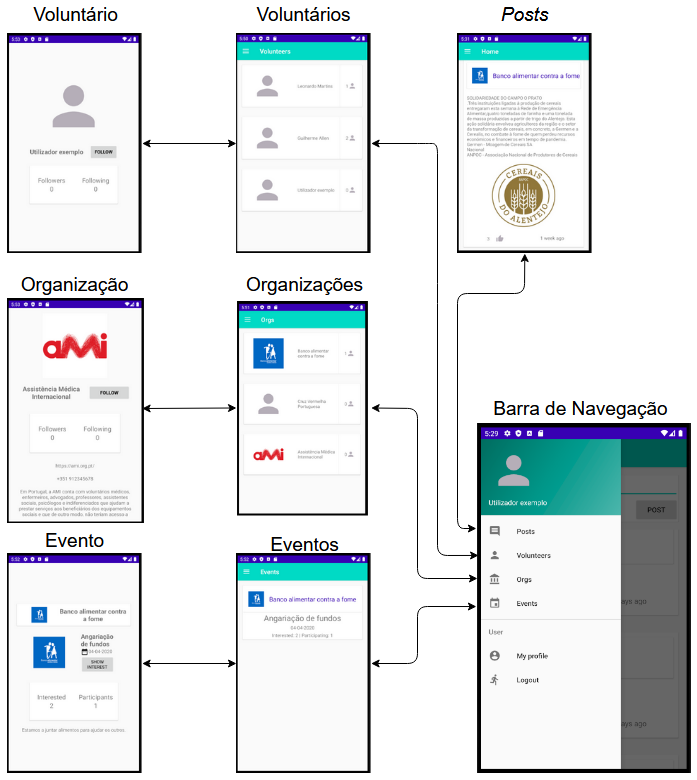
\includegraphics[scale=.65]{app_navigation.png}
	\caption{Grafo de navegação}
\end{figure}

Foram desenvolvidas quatro vistas principais de pesquisa (\textit{posts}, voluntários, organizações e eventos) que apresentam os dados existentes na plataforma. Existem também vistas detalhadas para estes mesmos índices (exceto \textit{posts}) para que o utilizador possa ver os detalhes destes dados.

\bigskip

\subsection{Sessão}

De maneira a garantir uma experiência personalizada para cada cliente deste módulo, foram desenvolvidos ecrãs e mecanismos de de registo e autenticação de clientes.

\begin{figure}[h]
	\centering
	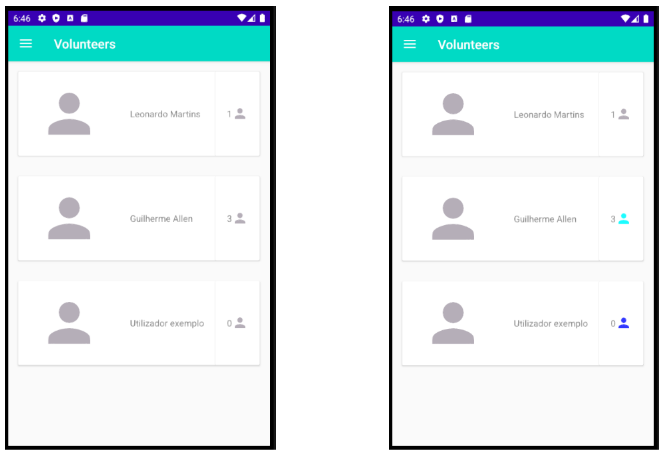
\includegraphics[scale=.70]{unauthenticated_vs_authenticated}
	\caption{Representação do ecrã ``Voluntários'' no estado não autenticado (esquerda) e no estado autenticado (direita) como o utilizador ``Utilizador exemplo''.}
\end{figure}

A partir do momento que um cliente da aplicação se encontre autenticado, certas operações como ``gostar'' um \textit{post} ou seguir um utilizador passam a estar disponíveis e determinados ecrãs irão ter uma vista personalizada, tal como exemplificado na Figura 7.

\subsection{Arquitetura}

Levando em consideração que este projeto utiliza o conjunto de guias dadas pelo Android Jetpack,
a arquitetura da aplicação é a recomendada e, como tal, é constituída por três sub-módulos principais: UI (User Interface), API e Modelo~\cite{AndroidJetpack2020}.

\medskip

Enquanto que a UI é responsável por conter as implementações dos mais variados aspetos da interface de utilizador (como atividades, fragmentos, navegação e outros elementos), a API trata a comunicação entre a aplicação e a Web API. Por fim, o Modelo define a estrutura dos dados fornecidos pela API e utilizados na UI assim como a implementação de uma \textit{cache} de maneira a partilhar estes dados e reduzir o número de pedidos efetuados à Web API.

\subsubsection{\textit{User Interface}}

Este sub-módulo engloba todos os componentes do projeto que são responsáveis por representar os dados da aplicação. Este é constituído por:

\begin{itemize}
	\item implementações de ecrãs, quer sejam atividades ou fragmentos. É de notar que para cada um destes existe associado um objeto ViewModel que é responsável por manter o estado dos elementos do ecrã e também por interagir com a API quando necessário; 
	\item adaptadores, infraestruturas responsáveis por auxiliar o processo de transformação de dados brutos numa representação dos mesmos. Estes adaptadores são utilizados em conjunto com o componente RecyclerView - utilizado para apresentar uma lista de elementos (como voluntários ou \textit{posts}) ao utilizador;
	\item Outros componentes utilitários, como por exemplo uma estrutura que auxilia o carregamento de imagens para a representação das mesmas.
\end{itemize} 

\subsubsection{API}

O sub-módulo API (Figura 8) serve como \textit{proxy} entre a aplicação e a Web API. Este dispõe de um serviço que disponibiliza todas as rotas acessíveis pelos voluntários e sobre o mesmo é possível solicitar a realização de pedidos à API (como a obtenção de voluntários ou o seguimento, por parte do utilizador autenticado, de uma organização). O mesmo é assíncrono e funciona à base de \textit{callbacks}.

\begin{figure}[h]
	\centering
	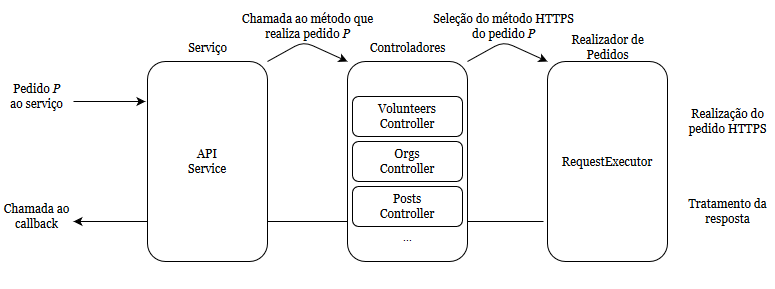
\includegraphics[scale=.42]{mobile_api_architeture}
	\caption{Arquitetura do sub-módulo API}
\end{figure}

O realizador de pedidos trata da implementação dos métodos HTTP suportados pela Web API (GET, POST, PUT, DELETE) de forma genérica, de maneira a que o mesmo possa ser utilizado pelos controladores. Os pedidos HTTPS são efetuados usando a biblioteca \textit{Volley}.

\medskip

Quando o pedido é concluído, é chamado o \textit{callback} definido pela estrutura que chamou o serviço, que consome a resposta do mesmo, quer esta contenha dados ou apenas sinalize sucesso. A estrutura que efetua a chamada ao serviço é também responsável por definir o \textit{callback} a executar em caso de ocorrer um erro durante o pedido.


\subsubsection{Implementação de Sessão}

Tendo em conta que o conceito de sessão foi implementado na Web API através da tecnologia Passport.js (que funciona à base de \textit{cookies}), foi necessário redefinir algumas infra-estruturas da biblioteca Volley de maneira a que, quando o utilizador estiver autenticado na aplicação, os pedidos efetuados pela mesma contenham a informação necessária para a Web API conseguir reconhecer o utilizador.

\medskip

De maneira a que a representação dos vários ecrãs da aplicação seja dinâmica consoante a sessão do utilizador, é definido e utilizado um objeto Sessão, acessível por todas as classes do projeto, que contém informações relativamente ao voluntário autenticado.

\subsubsection{Modelo}

O Modelo é responsável por transformar os dados provenientes do sub-módulo API para conjuntos de DTO (\textit{Data Transfer Object}) que irão ser usados pelo sub-módulo UI para efetuar a sua representação.

\medskip

Este sub-módulo contém também a definição de uma estrutura que realiza \textit{caching} dos dados da aplicação para diminuir o número de pedidos a realizar à API.